%!TEX root = ./main.tex
\section{Implementation}
\label{sec4}


We have implemented our resugaring approach using PLT Redex \cite{SEwPR}, a semantic engineering tool based on reduction semantics \cite{reduction}. We show several case studies to demonstrate the power of our approach. Some examples discussed in this section are in Fig. \ref{fig:resugaring}. Note that we set call-by-value lambda calculus as terms in \m{CommonExp}, because we want to output some intermediate expressions including lambda calculus in some examples. It is easy if we want to skip them.

\begin{figure}[t]
	\centering
	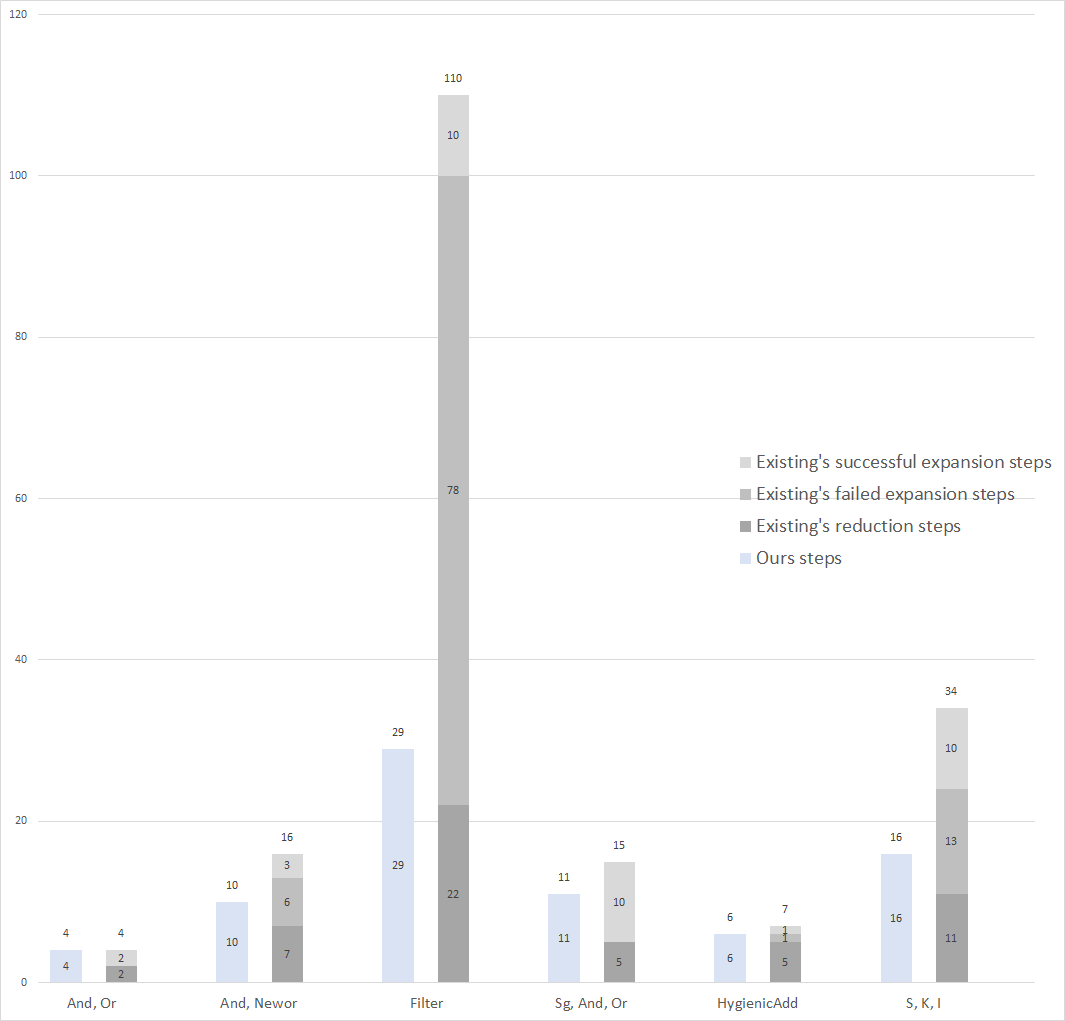
\includegraphics[width=0.47\textwidth]{images/efficiency.png}
	\caption{Comparison on Reduction Steps}
	\label{fig:step}
\end{figure}

To show the efficiency of our approach, we use the number of reduction steps comparing to the existing approach as the metrics. Figure \ref{fig:step} shows the difference between the two approaches. Notice that both approaches have pre-processing---for the existing one, it is to desugar the programs to the core language together with some tags; for ours, it is to calculate the context rules of syntactic sugars. We do not consider the steps during pre-processing. Besides, we derive the reduction steps of the existing approach into three different kinds---the reductions in the core language, the reverse expansion with failed resugaring, the reverse expansion with successful resugaring.  Use the following example to see the difference. Consider a sugar named \m{Hard} with two arguments, which has many reduction steps after desugared. Assuming for specific $e_1$ and $e_2$, the \Code{(Hard $e_1$ $e_2$)} after fully desugared has 100 reduction steps (finally to \#f, for example), and only 1 intermediate step can be resugared (to \Code{(Hard $v_1$ $e_2$)}, for example). Then for \Code{(And (Hard $e_1$ $e_2$) \#t)}, although all the 100 steps in the core language try the reverse desugaring, only \Code{(if stepn \#t \#f)} (2 steps on \m{And}, \m{Hard}) and \Code{(if \#f \#t \#f)} (1 step on \m{And}) are successful. Other 98 attempts will be failed together with 98 steps on \m{And}.

\[
{\footnotesize
	\begin{array}{lcl}
	Surface&&Core\\
	\Code{(And (Hard $e_1$ $e_2$) \#t)}&\xrightarrow{desugar}&\Code{(if step0 \#t \#f)}\\
	\qquad\quad\dashdownarrow& &\qquad\qquad\downarrow\\
	\Code{(And step1 \#t)}&\xleftarrow{resugar}&\Code{(if step1 \#t \#f)}\\
	\qquad\quad\vdots& &\qquad\qquad\vdots\\
	\Code{(And (Hard $v_1$ $e_2$) \#t)}&\xleftarrow{resugar}&\Code{(if stepn \#t \#f)}\\
	\qquad\quad\vdots& &\qquad\qquad\vdots\\
	\Code{(And \#f \#t)}&\xleftarrow{resugar}& \Code{(if \#f \#t \#f)}\\
	\qquad\quad\dashdownarrow& &\qquad\qquad\downarrow\\
	\Code{\#f}&& \Code{\#f}\\
\end{array}
}
\]


The general regularity is---the more complex the sugar is, the more steps will our approach save. Note that if the RHS of a syntactic sugar is huge, one-step reduction of the reverse desugaring will also be complex, because huge sugars will contain many failed attempts to resugar. So avoiding reverse expansion of syntactic sugar can improve the efficiency for practical use because programs are usually not that small like the demos.
